\subsection{Mechanics} \label{sec:mechanics}
In his work \citeauthor{Schell2014} discerns seven distinct mechanics which define what a game is in its core.
They can be seen as the skeletal frame of a game behind the curtain of aesthetics, technology and storytelling.
Game designers should be able to look behind this curtain and identify the main mechanics making up a specific game.
He argues that while their is no single standard taxonomy due to the inherent complexity and hidden structures it is worthwhile to work towards a common understanding.
Definitions should avoid both too much simplification and excessive precision.
In the end the classifications should work towards providing useful insights into games for designers \cite{Schell2014}.

\subsubsection{Space} \label{sec:space}
Thinking about the \textit{space} of a game requires an abstract, mathematical view which blanks out any visual aesthetics.
A game's space describes all possible places and their connection to each other.
They feature three main characteristics \cite{Schell2014}:
\begin{itemize}
    \item Discrete or continuous
    \item Number of dimensions
    \item Bounds and connections
\end{itemize}
\textit{Discrete} spaces are restricted to a finite number of places.
Board games commonly have this characteristic; even though pieces can be freely placed within the area of 2D boards (sometimes 3D) only a set of places carries meaning for the mechanics of the game.
Conversely, \textit{continuous} space can also be restricted in terms of its dimensions but elements are placed freely at any position.
Pong\footnote{\url{https://en.wikipedia.org/wiki/Pong}, Accessed: 01-03-2018} is a good example for a 2D playing field with continuous movement.
It recreates top-down table tennis with paddles on either side and a ball moving back and forth.
Both paddles are locked into vertical bounds but can have any arbitrary position within.

The previous characteristic already touched upon the \textit{dimensionality} of games.
Naturally, two dimensions (2D) and three dimensions (3D, reality) come to mind.
Information state can also be represented in an abstract space model.
Even when a game, like quiz games, might not feature a dimensional world the state of players exists in zero dimensional spaces.

Finally, the third characteristic is concerned with \textit{bounding areas} in spaces or if they are \textit{connected}.
The contrast is visible when thinking of bounded board games versus Pong again. 
Various places in a board game have limited areas where pieces can be placed.
Within this area positions carry the same meaning; borders to neighboring fields create a pathway through the game.
In Pong the areas are connected and allow for free movement of elements.

With these characteristics in mind complexity increases when nesting multiple spaces.
Nested spaces are not required to be of the same nature.
They are usually connected through special points which allow players to switch between spaces.
Role-playing games sometimes distinguish between outdoor and indoor spaces which can be changed by travelling through gateway icons \cite{Schell2014}.

\subsubsection{Time}
In reality \citeauthor{Schell2014} describes \textit{time} as a constant dimension which we cannot manipulate; it always moves forward at the same speed. 
Games empower us to change this force of nature at free will by either handing full control to the designer or directly to the player.

Similar to space, in the previous section (Section \ref{sec:space}), time is discrete, continuous or hybrid. Discrete time is found in turn-based games which consists of a series of turns without measured time.
Games in continuous time are not restricted to these turns which, in most cases, is more suitable for the action and sports genre.
Hybrid combinations are still based around turns and additionally measure or limit the continuous time in between.

Absolute and relative time limits are used to limit gameplay in different ways.
On a global scale clocks can limit the time a game can be played (e.g. soccer) and going into the details time limits can also limit the length of certain game mechanics (e.g. duration of jumps or attacks).
Once again with a similarity to space, (Section \ref{sec:space}) nested timers force players to make decisions and take risks.
These previous timers are usually absolute measures whereas relative time limits are commonly found in races.
Instead of having a fixed time limit relative timers create pressure by pushing players to be faster than something else (e.g. faster than other players).
Finally, time can also have an effect on physical or cognitive endurance which creates a different kind of limit.

Most games are equipped with some kind of mechanism to manipulate time.
Common examples include stopping time by pausing a game or going back in time to a checkpoint.
Furthermore, certain strategy games (e.g. Civilization, Anno, Kingdoms \& Castles, etc.) allow players to control the speed of time in order to create more dynamic.
Building games around the manipulation of time can serve as a powerful mechanic (e.g. Braid, Superhot).

\subsubsection{Objects, Attributes, and States} \label{sec:objects-attributes}
The space of a game is populated by objects which is anything that is visible or that can be manipulated \cite{Schell2014}.
Objects have one or more attributes attached which are pieces of information about the object itself.
Usually object have at least one attribute containing the position in the game space.
Every attribute has a current state which changes throughout the game.
The frequency of state changes depends on the nature of an attribute.
Velocity of an object dynamically changes with each update of the game loop whereas shape or color can be considered to be static properties (unless there are transformations to the object).
\citeauthor{Schell2014} uses the analogy of nouns and adjectives for objects and attributes respectively.

Designers have to think about which state changes are communicated to players.
It is possible that some changes should remain hidden for the sake of better gameplay or to prevent cognitive overload.
Therefore, designers should remember the interconnections of states.
However, the complexity easily explodes with more sophisticated games which is why diagrams of state machines can help to visualize these connections.

Secrets radically change game mechanics by restricting information access.
The opposite is found in board games which commonly have so called perfect information.
Every player is aware of all states except the other players thoughts.
Making groups of information either public or private creates a different kind of dynamic.
It adds the objective of obtaining private information of others to be used as an advantage.
This is possible by guessing or monitoring state changes and deriving conclusions.
Videogames introduce two state scopes: State information which virtual opponents are able to access and the game itself which inherently has access to all information.
Randomly generated information takes a special place because it cannot be known until it is generated (unless the game uses pseudorandomness).

\subsubsection{Actions}
If objects are the nouns and attributes the adjectives of game mechanics (Section \ref{sec:objects-attributes}) then \textit{actions} represent verbs \cite{Schell2014}.
Actions generally fall into one of two categories: Basic or strategic actions.
Base actions are the initial tool set of players, for example: Moving, jumping or interacting with other objects.
Using these tools players execute strategic actions to work towards achieving an objective, for example: Moving to the finish line, blocking opponents or avoiding obstacles.

Strategic actions enable emergent gameplay which is generally considered to be essential for interesting games.
It describes actions and strategies that are not explicitly defined by the game but rather emerge and evolve through playing the game.
Albeit being a subjective matter, the ratio between strategic actions to basic actions serves as an indicator for emergent gameplay \cite{Schell2014}.
However, emergent behavior is fragile in the sense of easily vanishing when basic actions are adjusted.
Therefore, designers need to recognize emergent strategies and pay attention to conserving the intricate effects of base actions.
Five guidelines potentially unlock emergent gameplay:

\begin{enumerate}
    \item Adding actions
    \item Actions on multiple objects
    \item Multiple ways to achieve goals
    \item Many objects
    \item Side effects
\end{enumerate}

(1) Firstly, adding more actions increases interaction which subsequently increases the opportunity for establishing emergent gameplay.
At the same time one should avoid cluttering games with a needless amount of actions.
Carefully crafted base actions with interesting interactions between each other and objects generally lead to better gameplay.

(2) Allowing actions to act on various objects gives freedom of choice to the player.
Moreover, it enables exploration of these different possibilities which in turn produces strategic actions.

(3) Providing players with a multitude of actions and objects to act on is only one part of the equation.
Dynamic gameplay can only exist if goals are reachable in different ways.
Otherwise players find themselves in a lock-in situation where choices does not contribute towards achieving objectives.

(4) This guideline does not necessarily add value to every game but is crucial for others.
Using board games, like chess, as an example managing a group of pieces enables players to sacrifice pieces or position them strategically.
The same principle is applicable for videogames where players manage worker or military units in various strategic ways.

(5) Finally, all actions taken by players produce more or less obvious side effects in a game's space.
This places constraints on both players and their opponents.
If, for example, units occupy space at their position this space is rendered unusable for any other unit in the game. Furthermore, every movement changes the constraint of occupied space dynamically.

\subsubsection{Rules} \label{sec:mechanics-rules}
\textit{Rules} are considered to be the most fundamental game mechanic essentially defining the goal and everything that is possible to achieve this goal \cite{Schell2014}.
Figure \ref{fig:rules} depicts David Parlett's analysis of eight different types of rules found in games.

\begin{figure}[H]
    \centering
    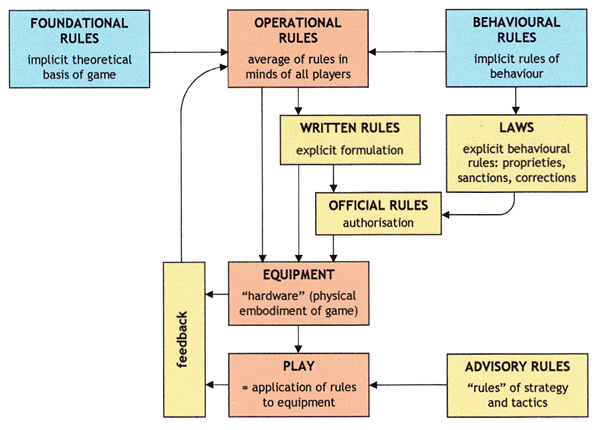
\includegraphics[width=8cm]{assets/rules.png}
    \caption{David Parlett's rule analysis\protect\footnotemark}
    \label{fig:rules}
\end{figure}
\footnotetext{\url{http://www.parlettgames.uk/gamester/rulesOK.html}, Accessed: 02-03-2018}

(1) Operational rules are everything a player needs to play a game.
They describe what is done to play the game.

(2) Foundational rules represent the underlying mathematical structure of the game.
Essentially breaking it down into states declaring when and how they change.


(3) Behavioral rules can be understood as the social contract when playing games.
Players intuitively understand these rules as fairplay which is why they are not written down.

(4) Written rules, in contract to behavioral rules, are explicitly manifested in documents that come with a game either physically or virtually.
Obtaining an understanding of the operational rules is achieved by reading the written rules, receiving explanations from others or simply by playing the game.
Due to the encoded nature of written rules most players tend to prefer different ways of learning.
They are exceptionally useful when players need to resolve conflicts and require a reference to neutral rules.

(5) Laws come into play during competitive tournaments.
They clarify or alter written rules and may include additional rules.
Modification or addition is mostly used to improve or balance games for serious scenarios.

(6) Official rules are the result of merging written rules and laws over time.
At some point they become the written rules again.

(7) Advisory rules assume a more strategic nature and boil down to advices helping players to perform better in a game.

(8) House rules are not included in Figure \ref{fig:rules} but are the result of the feedback loop.
Players may create their own set of rules to overcome deficiencies or to increase perceived fun.

Games are able to switch between different rule sets using modes.
Different modes alter parts of the existing rules or create sub-games with entirely new rules.
As players can get lost in these alternative modes they should be informed which mode is active and should not spend more time outside the main mode than inside.

Traditionally rules have been enforced by players or neutral referees in serious tournaments.
Computers can host much more complex games and automate the role of enforcing rules.
While this is powerful for creating rich games designers need to ensure that rules are intuitive for players.
Games should be designed in a way which allows players to test which things work and thereby discover rules naturally.

Cheating is the sole reason games require an enforcing instance for its rules.
Circumventing rules puts a player into a position of disproportional advantage which clearly satisfies the need for winning.
While this is a strong argument for enforcing rules already there is a more subtle effect at play as identified by \citeauthor{Schell2014}.
If a game is perceived as cheatable, whether that is actually the case or not, players might simply stop playing.
Investing time, effort and skill to work within the rules is rendered worthless by imagining someone potentially skipping these constraints.

Special attention should be payed to defining the main objective of a game. 
It can be considered the most important rule of all as it spurs motivation in players to achieve the defined goals \cite{Schell2014}.
Clearly defining all goals and how they relate to each other is essential for conveying the gist of a game in a well defined manner.
Only when players understand the objectives and are able to imagine ways ultimately achieving them they will feel an urge to play.
Three characteristics are shared by well-defined goals, they are: (1) Concrete, (2) achievable, and (3) rewarding.
It should be noted that these characteristics are not strict requirements and that they do not always have to be in perfect equilibrium.
Games can certainly be build around the exploration and discovery of the main objective (e.g. The Stanley Parable).
The same principle applies to achievable goals for a range of games centered around frustration and requiring excellent coordination to solve objectives (e.g. QWOP, Dark Souls series, Super Meat Boy).
Instead of players expressing resentment they manage to trigger an even stronger reverse effect of numerous attempts to beat the game.
This might be due to the goal still being concrete (e.g. finish all levels) and the perceived reward seeming particularly special as only a few players manage to finish these games.

\subsubsection{Skill} \label{sec:skill}
\textit{Skill} is a mechanic which games demand from players.
Matching a game's difficulty with the player's skill set creates a challenge; otherwise the game will be perceived as being too easy or too hard.
Naturally, more than a single skill is expected from players which generally stems from three main categories \cite{Schell2014}:

\begin{enumerate}
    \item \textbf{Physical:} Strength, dexterity, coordination, and physical endurance
    \item \textbf{Mental:} Memory, observation, puzzle solving, and decision making
    \item \textbf{Social:} Reading opponents, fooling opponents, communication, and coordination within teams
\end{enumerate}

It is important to stress that these skills refer to real-world abilities.
Whereas videogames often feature virtual character skills these a merely attributes which can be improved by providing the correct input to the game.
Nonetheless, this requires a level of physical coordination for using the input device and following a strategy allowing to improve virtual skills (cognitive work).

Actually defining the required skills for a game is useful to reflect about the design but also proves to be surprisingly difficult.
It is easy to think that a single skill is essential for performing well in a game.
In reality many factors are in play deciding which final blend of skills are actually necessary.
They can deviate far from what a designer might envision initially.

\subsubsection{Chance}
The final game mechanic \textit{chance} exerts a strong influence on all previously discussed mechanics.
There are many games not relying on chance as a game element, for example chess.
While players can only assume what the next move of their opponent will be (with the exception of \textit{zugzwang}) there is no uncertainty involved in actually executing moves.
Virtually every possible move could be calculated and pre-planned at any given point in time.
Introducing chance into games changes this property which in its essence leads to surprises \cite{Schell2014}.
With uncertain outcomes in games skills (Section \ref{sec:skill}) and chance start to influence each other.

Firstly, the ability to estimate chances is a mental skill.
Understanding and keeping track of probabilities through the course of a game can greatly improve the advantage of a player.
It does not equal perfect prediction of the future but if a player is aware of probabilities a successful outcome is much more likely.

Furthermore, skills themselves underlie probabilities meaning that every action involves risk.
Circling back to the example of chess not exhibiting randomness this changes when taking the perspective of a player.
Basic actions like moving a piece on the chess board are not affected by uncertainty whereas strategic actions definitely involve risk and a chance of success.
Trying to lead the opponent into a desired situation can go unnoticed with a certain probability which depends on the opponent's skill level.

Consequently, the ability to assess an opponent' skill is a mental skill too.
It is crucial for making decisions which course of action to take which depends on chances of success.
As a form of emergent behavior it can be useful for players to trick opponents into assuming a lesser or greater skill level than what they are actually capable of.

Players need to remember that predicting the chance of independent events is a purely imagined skill \cite{Schell2014}.
This behavior is commonly exhibited in the ``luck streak fallacy'' and ``gambler's fallacy''.
The second fallacy already suggests that this mistake is usually made in gambling games where the chance of an event stays the same (e.g. Roulette, whether the ball lands in black or red).
Game designers can try to take advantage of these fallacies to steer players towards making the desired choices.
Likewise, the assumption that pure chance can be influenced is false.
At the same time it is important to understand that if a game of pure chance is broken down to a series of isolated events which cannot be influenced most players will not experience fun.